% -----------------------------------------------------------------------
% -----------------------------------------------------------------------
% -----------------------------------------------------------------------
% Einleitung
% -----------------------------------------------------------------------
% -----------------------------------------------------------------------
% -----------------------------------------------------------------------
\chapter{Introduction}

\section{Motivation: An Open-Domain Comparative Argumentative Machine (CAM)}


The topic of this master thesis is \emph{Argument Mining}, more precisely \emph{Comparative Argument Mining}. Argument Mining is an area in Natural Language Processing which gained popularity quite recently. The first workshop organized by the \emph{Association for Computational Linguistics} (ACL) was just hold three years ago, in 2014 (\cite{W14-21:2014}).\\
The aim of Argument Mining is the analysis of arguments in natural language. One can identify three main tasks: the identification of argumentative sentences, the components of an argument and their relations (cite). There are several definitions of the term \emph{argument} and it's structure (see section \ref{sec:argth}). In Argument Mining, the Claim/Premise model is often used. A claim is the statement of a sentence which is supported or attacked by one or more premises. An argument of this structure may look like the following:
\begin{quote}
    [X will win$]_{claim}$ [because$]_{support}$ [X can do Y$]_{premise}$
\end{quote}
The knowledge obtained by analyzing such sentences can be used \ldots\newline

Comparative Arguments are a special kind of arguments. The claim of a comparative argument is a comparison between one or more objects. The comparison frequently contains a direction (or polarity) in a sense that \emph{A is better / worse than B}.




\section{Applications}
\label{sec:applications}
A lot of

\section{Related Work}
\subsection{Argumentation Theory}
\label{sec:argth}
\subsection{Argument Mining}
\label{sec:argmine}
To my knowledge, there is no work dealing with Comparative Argument Mining (CAM) without domain restrictions. However, there is a lot of work on Argument Mining in general.\newline

Recent work in CAM was presented in \cite{gupta2017identifying}. In this paper, \emph{syntactic dependency graphs} were used to obtain patterns of comparative sentences. A restriction on the sentence was that both entities must be known (implicit comparisons are out of scope).  The rules were applied to the tasks of identifying comparative sentences (F1 score 0.87), the compared aspect (0.78), the scale indicator (like "lower"; F1 score 0.81 ) and the compared entities (0.77). The evaluation was performed on 189 comparisons extracted from 125 abstracts from papers of the bio-medical domain. \newline

Work on identifying argumentative sentences, their components and relations is also beneficial to this thesis, as some features and methods might be reused. An overview of features for those tasks was given in \cite{Aker2017What-works-and-}. Features and their combinations which were used in several other papers published between 2011 and 2015 were evaluated by the authors. To perform the experiments, several classifiers, ranging from simple linear models as Logistic Regression to Convolutional Neural Networks were used. 
Structural features were reported as most useful for argumentative sentence detection whereas \emph{syntactic features} were the least useful ones (in contrast to \cite{gupta2017identifying}, were syntactic dependency was used successfully). No classifier clearly outperformed all others, yet Random Forests were best in one corpus and comparable to the rest on the other one.\newline

The concept of claims was analyzed for six data sets in \cite{Daxenberger2017What-is-the-Ess}. The intention was to test how different conceptualization of claims impairs their classification. In cross-domain experiments, classifiers were trained on one full dataset (source domain) and tested against the other datasets (target domain). Featured-based approaches with all features outperformed the deep learning approaches in most combinations. Additionally, in-domain experiments on one dataset (10-fold cross-validation) were conducted. Here, Logistic Regression with syntax features gave the best results. Also, lexical and embedding features were useful.\newline


User-generated web discourse was used as the data source in this thesis. Therefore, it is valuable to review articles which handle this kind of data.
Argument mining for twitter data is performed in \cite{Dusmanu2017Argument-Mining}. In addition to find argumentative tweets, the authors try to distinguish factual arguments from personal opinion and find the source for the first one. Since tweets are short and user-generated, this can provide some insights for this thesis. For the task of argument identification, a F1 score of 0.78 is reached using Logistic Regression. As in \cite{Daxenberger2017What-is-the-Ess}, \emph{lexical features} (unigrams, bigrams and WordNet verb synsets) where quite powerful: Logistic Regression with lexical features produced a F1 score of 0.73.\newline

%Papers I think are interesting because of features used
In \cite{Wachsmuth2017Building-an-arg}, a basic framework for argument search engines is created. A common data structure for arguments is developed which makes it possible to transform different argument concepts into it. The prototype\footnote{Available at: http://www.args.me (Last checked: xx.xx.xxxx)} is also capable of retrieving competetive arguments.



\subsection{Domain-Specific Comparative Systems}
The enormous amount of Comparison Portals shows the need for comparisons. Television spots with high production value empathize the popularity of those portals.

Most of those portals are specific to a few domains and a subset of properties, for example, car insurances and their price. Because of that, those systems have some restrictions. Comparisons are only possible between objects of the domains and predefined properties. Source of the data is usually databases. Humans are involved in gathering, entering and processing. 

Comparison Portals solely compare and deliver facts. Because of that, they can only give the advice to choose X over Y based on the facts collected.  An insurance X might be the best in the comparison (e.g., best price), while the internet is full of complaints about lousy service.\newline

Examples of classical Comparative Portals are \emph{Check24, Verivox, Idealo, GoCompare,} and \emph{Compare}\footnote{https://check24.de, https://verivox.de, https://idealo.de, https://gocompare.com, https://compare.com - all last checked: 12.12.2017}, just to name a few.

As an example, Check24. can compare a wide variety of different objects like several insurance types, credit cards, energy providers, internet providers, flights, hotels and car tires. After the user entered some details (based on the object type, see figure \ref{img:check24}), Check24 shows a ranking of different service providers. The user can choose different properties to re-rank the list.
For instance, to compare different DSL providers, the user has to enter her address, how fast the internet should be and if she wants telephone and television as well. She can then select price, speed, and grade (rating) to sort the resulting list.

\begin{figure}[h]
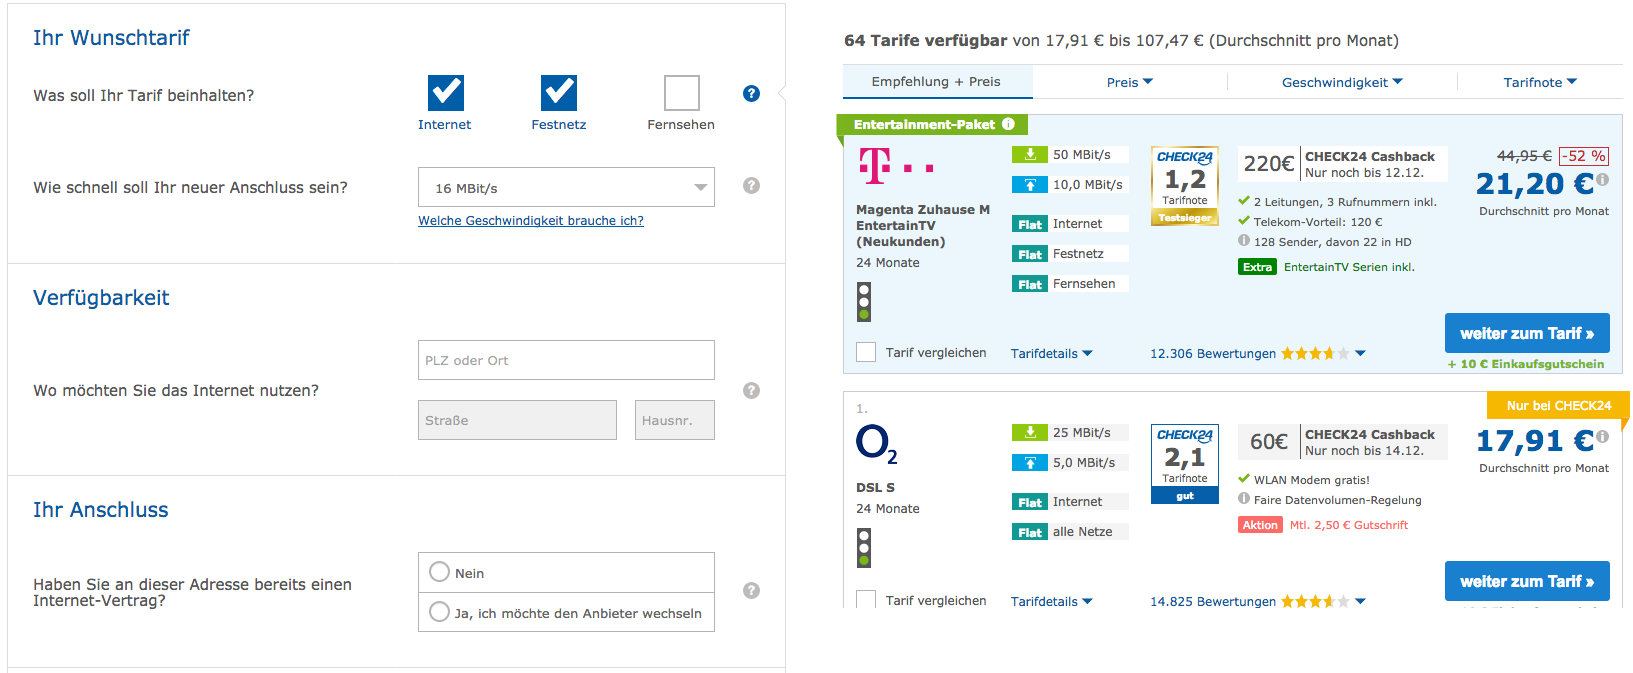
\includegraphics[width=1\textwidth]{images/ds-sys/check24}
\label{img:check24}
\caption{Check24 DSL Provider}
\end{figure}
The other mentioned sites work similarly. They provide more of a ranking than a comparison.\newline


Another interesting type of websites are Question Answering Portals like \emph{Quora} or \emph{GuteFrage}\footnote{https://quora.com, https://gutefrage.net - all last checked: 12.12.2017}. Although comparisons are not their primary goal, a lot of comparative questions are present on those sites.
On Quora, more than 2.380.000 questions have the phrase \enquote{better than} in their title. If \emph{Ruby} and \emph{Python} are added, 10.100 questions remain.\footnote{Checked via Google on 11th of December. Search phrase: \texttt{"better than" site:quora.com} and \texttt{ruby python "better than" site:quora.com}}
Same is true for the German site GuteFrage, though, the numbers are smaller than on Quora.\footnote{334.000 for \texttt{"besser als" site:gutefrage.net} and 78 for \texttt{ruby python "Besser als" site:gutefrage.net}}\newline

More interestingly are systems which can compare any objects on arbitrary properties. Two examples are \emph{Diffen} and \emph{Versus}\footnote{https://diffen.com, https://versus.com - all last checked: 12.12.2017}.

Versus aggregates different freely available data sources like Wikipedia and official statistic reports. For example, the comparison of \enquote{Hamburg vs. Berlin} uses Wikipedia for the number of universities, worldstadiums.com for the availability of sport facilities and the Economist for the Big Mac Index. Presumably, some human processing is involved as the possible comparisons are limited. For instance, a comparison of Hamburg and Darmstadt is not possible as Darmstadt is not available on Versus. Likewise, \enquote{Ruby vs. Python} is not possible, Versus suggests to compare \enquote{Rome vs. Pyongyang} instead. Although Versus shows how many users \enquote{liked} the objects, it does not give a clear statement which one is better. For instance, it is not possible to check automatically whether Hamburg or Berlin is better for a short city trip. The user must search manually all valid properties like the number of museums, theaters, the price of public transport tickets and so on.

Similar to Versus, Diffen aggregates different data sources (see figure \ref{img:diffversus}). All in all, the aggregated information is similar to Versus. The comparison is also tabular. Besides the automatically aggregated data, users can add more information on their own. Diffen describes itself as \enquote{inspired by Wikipedia}\footnote{https://www.diffen.com/difference/Diffen:About - Last checked: 11.12.2017}. Diffen does not enforce any restrictions on the objects of comparison, but it faces the same problem as Versus: objects are missing. A comparison between Darmstadt and Hamburg is likewise not possible: all cells for Darmstadt in the table are just empty.\newline

\begin{figure}[h]
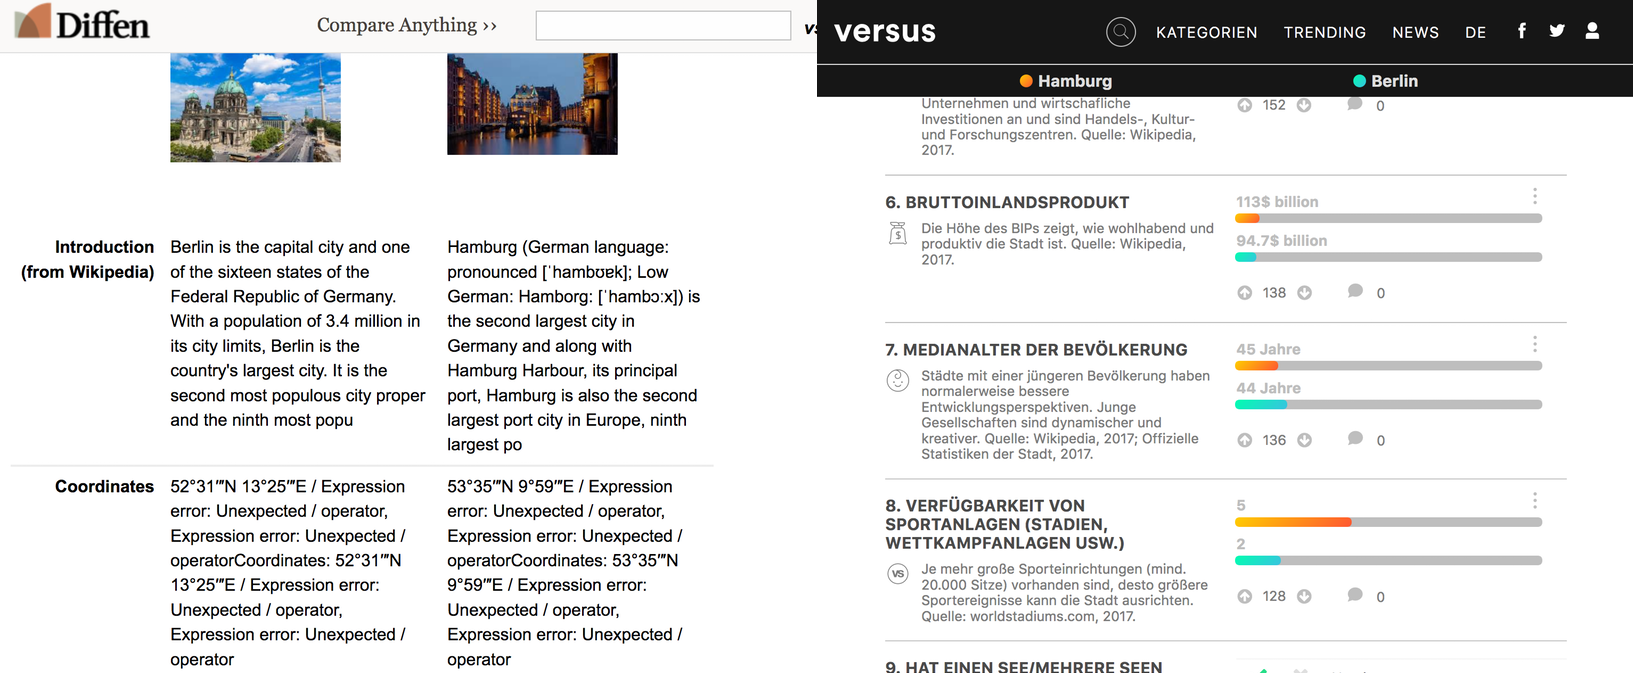
\includegraphics[width=1\textwidth]{images/ds-sys/diffversus}
\label{img:diffversus}
\caption{\enquote{Hamburg vs. Berlin} on Diffen and Versus}
\end{figure}

Neither Versus nor Diffen provides a comprehensible reason why an object is better than another one. They merely aggregate facts and bring them face to face. Despite the aggregation approach of both systems, many meaningful comparisons are not possible or not helpful (\enquote{Hamburg vs. Darmstadt}, \enquote{Java vs. C\#}, \enquote{Dr Pepper vs. Orange Juice}).
Also, the user can not define the properties for the comparison. The sites provide every information available for the objects. For instance, Versus shows 42 properties for \enquote{Hamburg vs. Berlin} and only 35 for \enquote{Hamburg vs. Munich}.
\newline

To summarize, a lot of different comparison portals exist and are widely used. Especially the domain-specific portals do a good job, but inflexibility dearly buys the performance. First, the portals can only compare objects on predefined properties. Second, the data acquisition is not fully automatic. Domain-unspecific systems are good at aggregating information but do not provide a reasonable explanation to prefer X over Y.

Adding information like comments and product reviews can enrich the comparison with reasons and opinions, such as \enquote{Ruby is easier to learn than C} or \enquote{Python is more suitable for scientific applications than Erlang as many libraries exist}.